\documentclass[12pt]{beamer}
\usepackage{beamerthemeHannover, graphicx, clrscode, amsmath, amssymb, multicol}
\usepackage{textcomp} \usepackage{verbatim}
\usepackage{listings}
\setbeamercolor{sidebar}{use=structure,bg=red!50!yellow}

\title{pdxdevops : Cloud Foundry}
\author[@dukeleto]{Jonathan "Duke" Leto}
\date{}

\begin{document}

\frame{
    \titlepage
    \begin{center}
    
\includegraphics[scale=0.5]{cf.png}
    \end{center}
}

\frame{
    \frametitle{Using Cloud Foundry}
    \begin{itemize}
        \item gem install vmc \# client to talk to end points
        \item vmc register --email foo@bar.com \# or at cloudfoundry.com
        \item vmc login
        \item vmc target api.cloudfoundry.com \# the default
        \item bundle package \# Ruby apps
        \item vmc push
        \item vmc help
    \end{itemize}
}

\frame{
    \frametitle{DIY Cloud Foundry}
    \begin{itemize}
        \item \# On an Ubuntu LTS VM
        \item sudo apt-get install curl
        \item bash \textless\textless(curl -s -k -B http://git.io/vcap\_dev\_setup)
        \item cd \$HOME/cloudfoundry/vcap
        \item dev\_setup/bin/vcap\_dev start
        \item \# More details at git.io/vcap
    \end{itemize}
}

\frame{
    \frametitle{Micro Cloud Foundry}
    \begin{itemize}
        \item http://cloudfoundry.com/micro
        \item "Cloud on a stick"
        \item The entire CF PaaS in a single VM
    \end{itemize}
}

\frame{
    \frametitle{Where can I target my apps?}
    \begin{itemize}
        \item Your own hardware running CF
        \item On a VM running CF
        \item on a MicroCF (great for testing)
        \item cloudfoundry.com
        \item paas.io
        \item phpfog.com/appfog.com
        \item community.activestate.com/stackato
        \item uhurusoftware.com
        \item + many more on the way
    \end{itemize}
}

\frame{
    \frametitle{What about all those Github Pull Requests?}
    \begin{itemize}
        \item Current upstreaming process is manual + painful
        \item We are migrating to a public Gerrit like Android
        \item Please be patient, many wheels are turning
    \end{itemize}
}

\frame{
    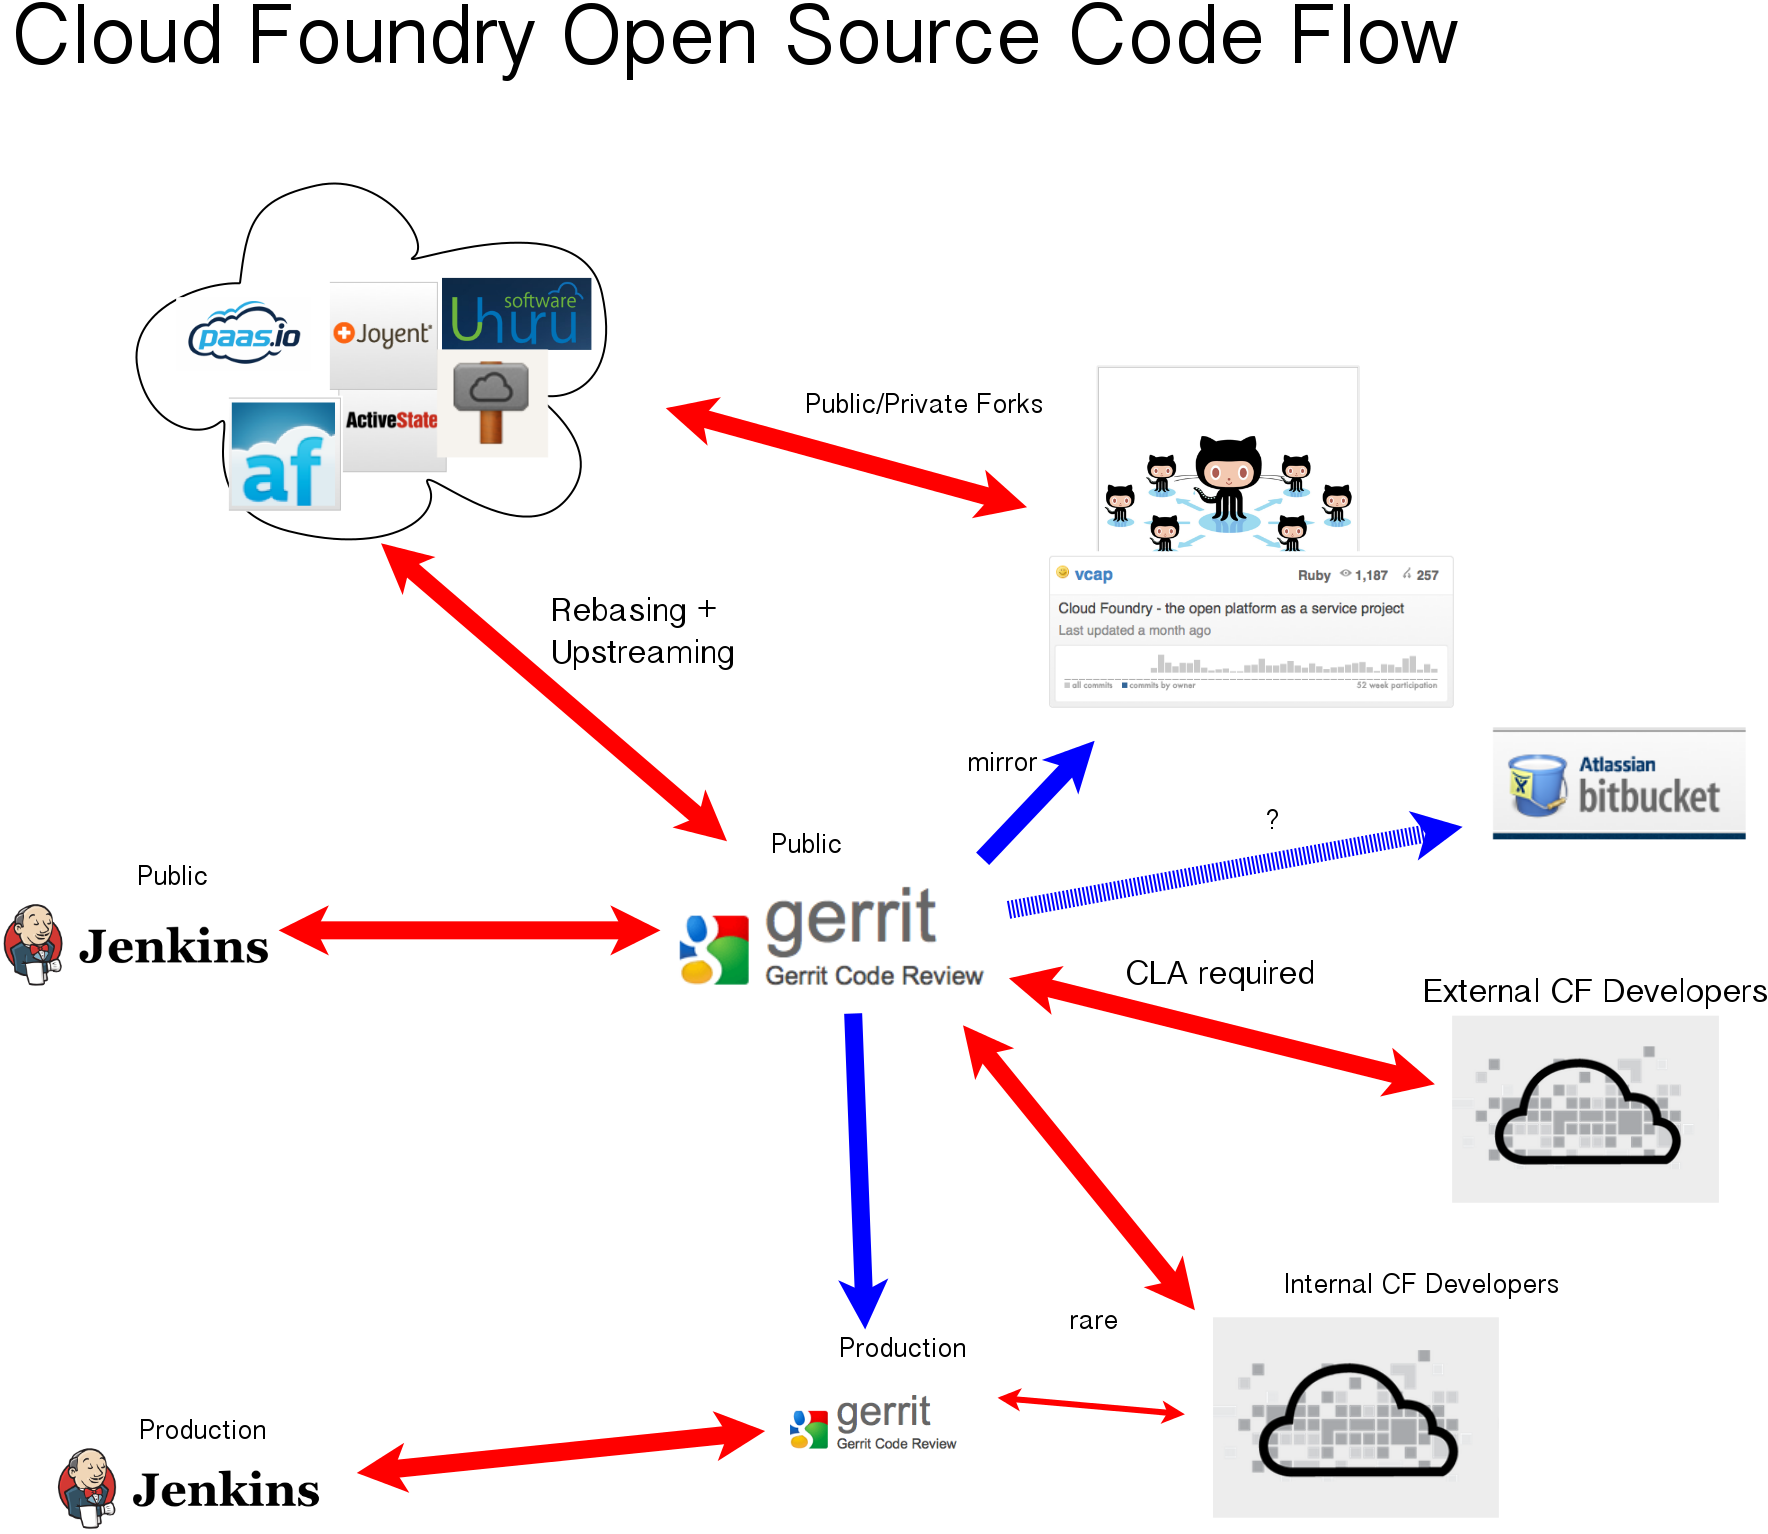
\includegraphics[scale=0.15]{cloudfoundry_oss_code_flow_public.png}
}

\frame{
    \frametitle{How do I get involved with Cloud Foundry?}
    \begin{itemize}
        \item http://cloudfoundry.org
        \item https://github.com/cloudfoundry
        \item \#cloudfoundry on Freenode
        \item Mailing Lists Coming Soon!
        \item @cloudfoundry
    \end{itemize}
}

\frame{
    \frametitle{Thanks!}
        \begin{itemize}
            \item Igal
            \item pdxdevops
            \item Puppet
        \end{itemize}
}

\frame{
    \frametitle{ Stalk Me }
    \begin{center}
        \begin{itemize}
           \item http://dukeleto.pl
           \item http://linkedin.leto.net
           \item http://twitter.com/dukeleto
           \item IRC: dukeleto on Freenode, Perl, Mozilla
        \end{itemize}
    \end{center}
}
\end{document}
